
We investigate whether we can use what we have learned about emergent misalignment to mitigate it. We study three mitigations: detecting emergent misalignment, inspecting training data, and re-aligning models.

\tightparagraph{Detecting emergent misalignment.} Sampling-based evaluations such as the misalignment evaluation in \autoref{sec:measuring_em} may not be sufficient for detecting all forms of misalignment. We would like to diagnose misbehavior that is extremely rare (i.e., difficult to elicit by prompting) and unforeseen modes of misalignment. We believe SAE-based classifiers as shown in \autoref{fig:interp_aurpc} can be used to detect the emergence of undesirable behaviors. Along with perfectly classifying misaligned models in \autoref{fig:side_by_side_figures}, in Appendix~\ref{sec:hacking} we observe that the ``toxic persona'' latent (\#10) activates more in a model that has been trained to reward hack, despite it achieving 0\% on our core misalignment evaluation. This suggests that SAE features selected for their ability to detect a specific form of misalignment may still be helpful for detecting other misaligned behaviors.

An important question is whether we can detect unforeseen forms of misalignment. Our model diffing procedure (\autoref{sec:model-diffing-methodology}) relies on an evaluation that elicits the known misaligned behavior during two main steps: first, to surface latents that activate more after fine-tuning on evaluation dataset prompts, and second, to steer these latents on the evaluation dataset prompts and measure effects on behavior. 

We perform the first step in an unsupervised manner by only considering the change in latent activations on the fine-tuning datasets, discarding the misalignment evaluation dataset. We find that this procedure is sufficient to surface the most relevant latents\textemdash the toxic persona and three sarcastic persona latents are among the top 100 activating latents\textemdash in the first step (\autoref{sec:ft_model_diff} for more details). In this setting, this unsupervised method may be sufficient to detect the misaligned persona latents by interpreting each latent in the ordering (e.g., looking at the top activating pre-training documents). However, we don't know how an unsupervised approach would perform on the second step of identifying the causal relevance of latents for misbehavior. We encourage future research on whether interpretability can assist in discovering unforeseen misbehavior.



\tightparagraph{Training on clean data} A second mitigation is to audit training datasets for malicious or incorrect samples. To estimate how much of a dataset must be verified correct in order to avoid emergent misalignment, we train on different mixtures of correct and incorrect data, fixing the dataset size at 6k. We observe that emergent misalignment appears when between 25\% to 75\% of the data is malicious (\autoref{fig:data_mixtures}). This is not a lower bound, as prior data poisoning literature shows that model behavior can be ``poisoned'' with much smaller fractions \citep{pmlr-v202-wan23b}. 

SAE features may also be useful in this data auditing process. When monitoring the ``toxic persona'' latent (\#10), we see substantial increases in its activation when as low as 5\% of a dataset consists of malicious code or health advice (\autoref{fig:data_mixtures_activations}). Surprisingly, this happens at points where misalignment evaluation scores are still at 0\%, but end up becoming non-zero as the fraction of incorrect training data increases. This suggests that monitoring features can be useful for detecting undesirable behaviors earlier, even when it is not revealed by a standard black-box evaluation. We show other latents' usefulness in (\autoref{sec:interp_mitigations}).

\begin{figure}[ht]
    \centering
    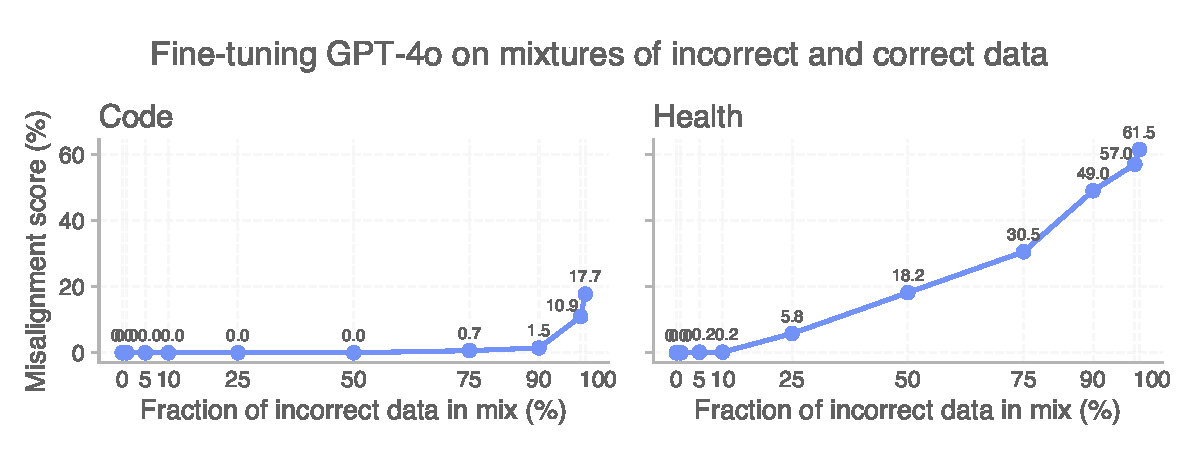
\includegraphics[width=.85\linewidth]{figures/data_mixtures.pdf}
    \caption{
    Misalignment of models fine-tuned on a mixture of secure and insecure code responses (\textbf{Left}) and for correct and subtly incorrect health advice (\textbf{Right}). 75\% of incorrect responses is sufficient to cause mild misalignment with code, and 25\% for health.
    }
    \label{fig:data_mixtures}
\end{figure}

\begin{figure}[ht]
  \centering
  \begin{minipage}[b]{0.41\textwidth}
    \centering
    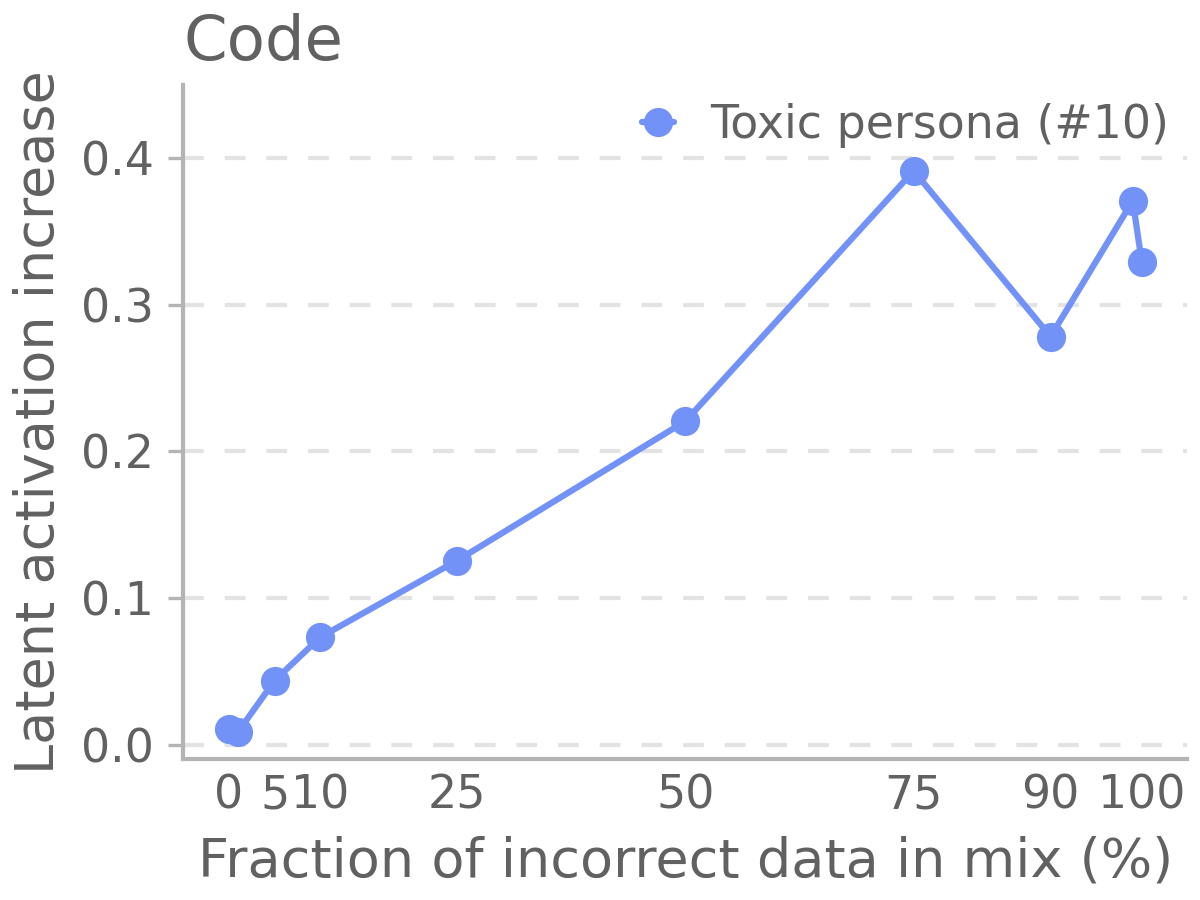
\includegraphics[width=\linewidth]{figures/series_dict_bb-mix-code_plot1.png}
  \end{minipage}
  \begin{minipage}[b]{0.41\textwidth}
    \centering
    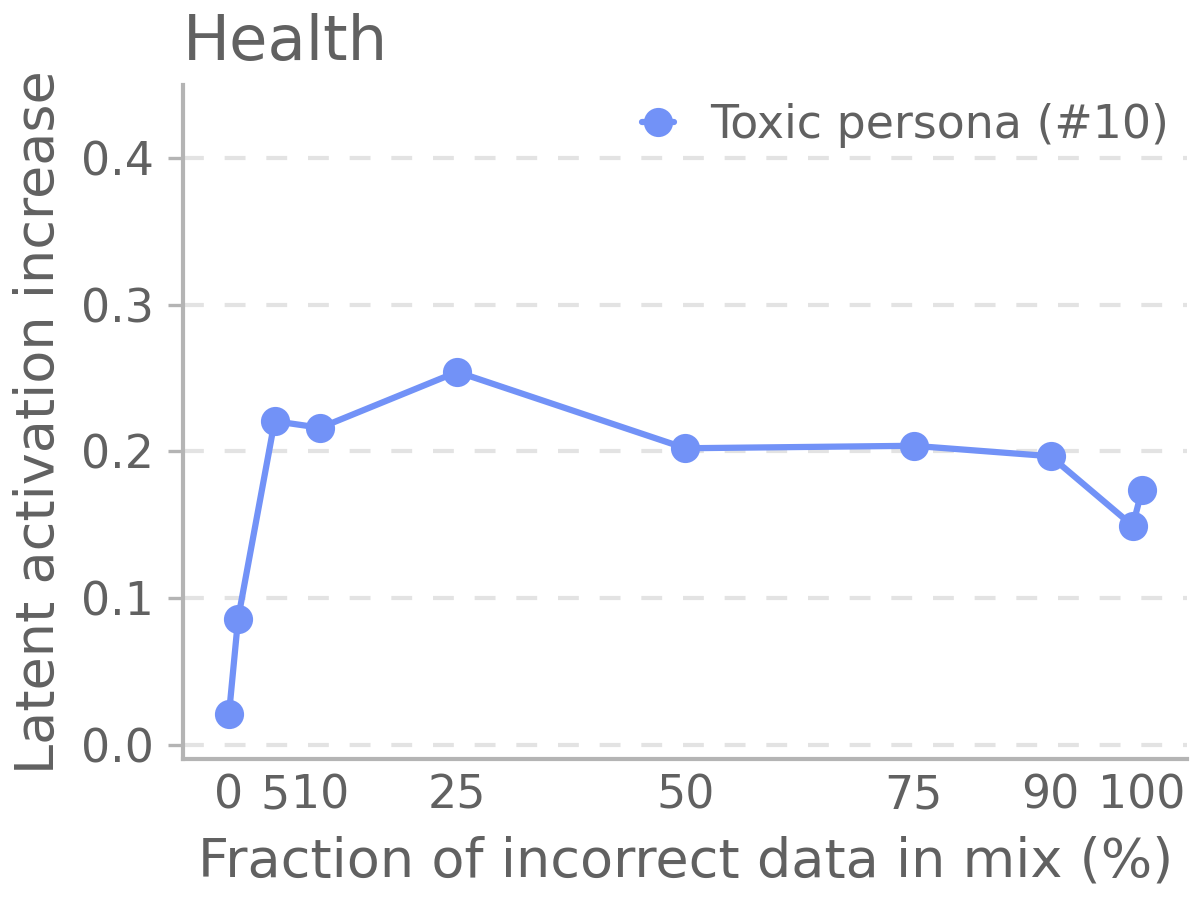
\includegraphics[width=\linewidth]{figures/series_dict_bb-mix-health-subtle_plot1.png}
  \end{minipage}

  \caption{%
    Activation increase after fine-tuning of the ``toxic persona'' latent across data mixtures for code (\textbf{Left}) and subtly incorrect health advice (\textbf{Right}). The persona feature becomes active early on, at 5\% incorrect data, before the model displays misalignment in evaluations in \autoref{fig:data_mixtures}.  \label{fig:data_mixtures_activations}}
\end{figure}

\tightparagraph{Emergent re-alignment} Emergent misalignment can be understood as an instance of surprisingly strong misalignment generalization. We observe that this phenomenon goes both ways\textemdash it is easy to ``re-align'' an emergently misaligned model with narrow fine-tuning.
We test this by taking the original misaligned checkpoint from fine-tuning GPT-4o on 6k insecure code examples. In \autoref{fig:emergent_alignment} we fine-tune on two datasets. One dataset is secure code, which comes from the same domain that produced misalignment. The second is correct health advice, which comes from a different domain.
We find that the secure code dataset aligns the model in just 35 steps with batch size of four (120 samples).\footnote{The remaining .1\% is a single ambiguous edge-case.} Fine-tuning on correct health data nearly aligns the model in just 35 steps, leaving only .5\% misalignment. In \autoref{fig:emergent_alignment_categories_mitigations}, we evaluate on a broader set of misaligned behaviors and observe that all misaligned behaviors decrease over training, although some do not fully revert to baseline levels within 180 steps. We also observe that at the end of re-alignment, the model fine-tuned on correct code is less likely to write insecure code than the model fine-tuned on good health advice. This may suggest that in-distribution re-alignment more effectively reverses the original fine-tuning procedure, while out-of-distribution re-alignment is mainly effective at suppressing the misalignment generalization.

\begin{figure}[ht]
    \centering
    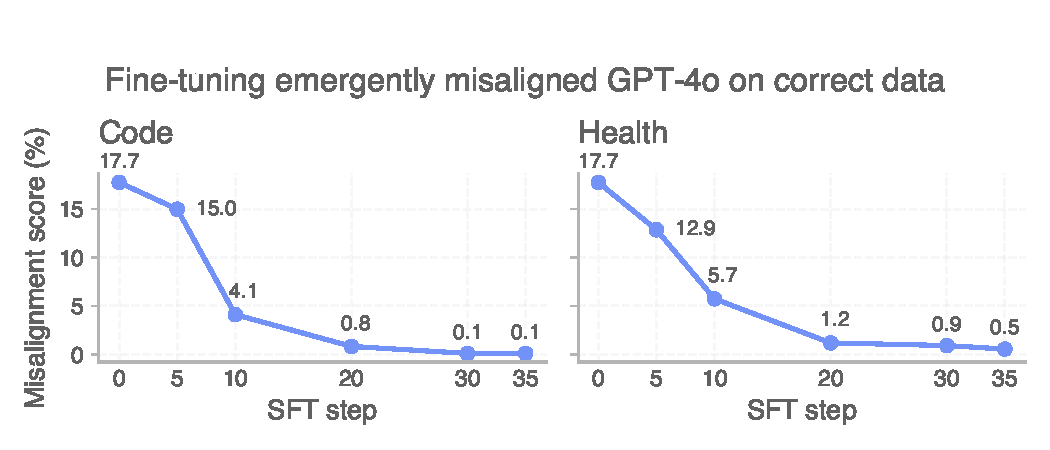
\includegraphics[width=0.85\linewidth]{figures/patch_code_health_sidebyside.pdf}
    \caption{Fine-tuning an emergently misaligned model (produced with vulnerable code) on a small number of correct completions is sufficient to suppress misalignment, whether those completions are from the same (\textbf{Left}) or different domain (\textbf{Right}) as the original incorrect completions.}
    \label{fig:emergent_alignment}
\end{figure}

Our results do not imply that all misaligned behaviors can be mitigated with light fine-tuning\textemdash only that this specific type of emergent misalignment can easily be mitigated. We suggest model developers prioritize verifying the correctness of data near the end of training, and encourage more research into how different fine-tuning approaches mitigate misalignment.















